\documentclass{article} 

\usepackage[hyphens]{url}
\usepackage[utf8]{inputenc}
\usepackage{hyperref}
\usepackage{longtable}
\usepackage{graphics,color}
\usepackage{amstext}
\usepackage{fullpage,epsfig}
\usepackage{verbatim}
\usepackage{hyperref}
\usepackage{enumerate}
\usepackage{xspace}
\usepackage{setspace}
\usepackage[utf8]{inputenc}
\usepackage[parfill]{parskip}
\usepackage{grffile}
\usepackage{lmodern}
\usepackage[T1]{fontenc}
\usepackage{textcomp}


\newcommand{\filefont}[1]{{\fontfamily{pnc}\selectfont #1}\xspace}
\newcommand{\nutemma}{\href{http://davids24.triumf.ca/~oliver/NUTEMMA/home.html}{\textcolor{blue}{NuTemma}}\xspace}
\newcommand{\hrefcolor}[2]{\href{#1}{\textcolor{blue}{#2}}\xspace}


\title{Geant4 EMMA (G4EMMA) Simulation Documentation\\
Version 1.8}
\author{Alex Wen, with (marked) sections by Naomi Galinski\\
taken from previous documentation}
\date{July 2017}

\usepackage{natbib}
\usepackage{graphicx}

\begin{document}

\maketitle

\clearpage

\tableofcontents

\clearpage

\section{Introduction}
The electromagnetic mass analyzer, or EMMA, is a recoil mass spectrometer (fig. \ref{EMMA}). It separates recoils from collisions between TRIUMF's ISAC II rare-isotope beam and a stationary target. 

\begin{figure}[h!]
\centering
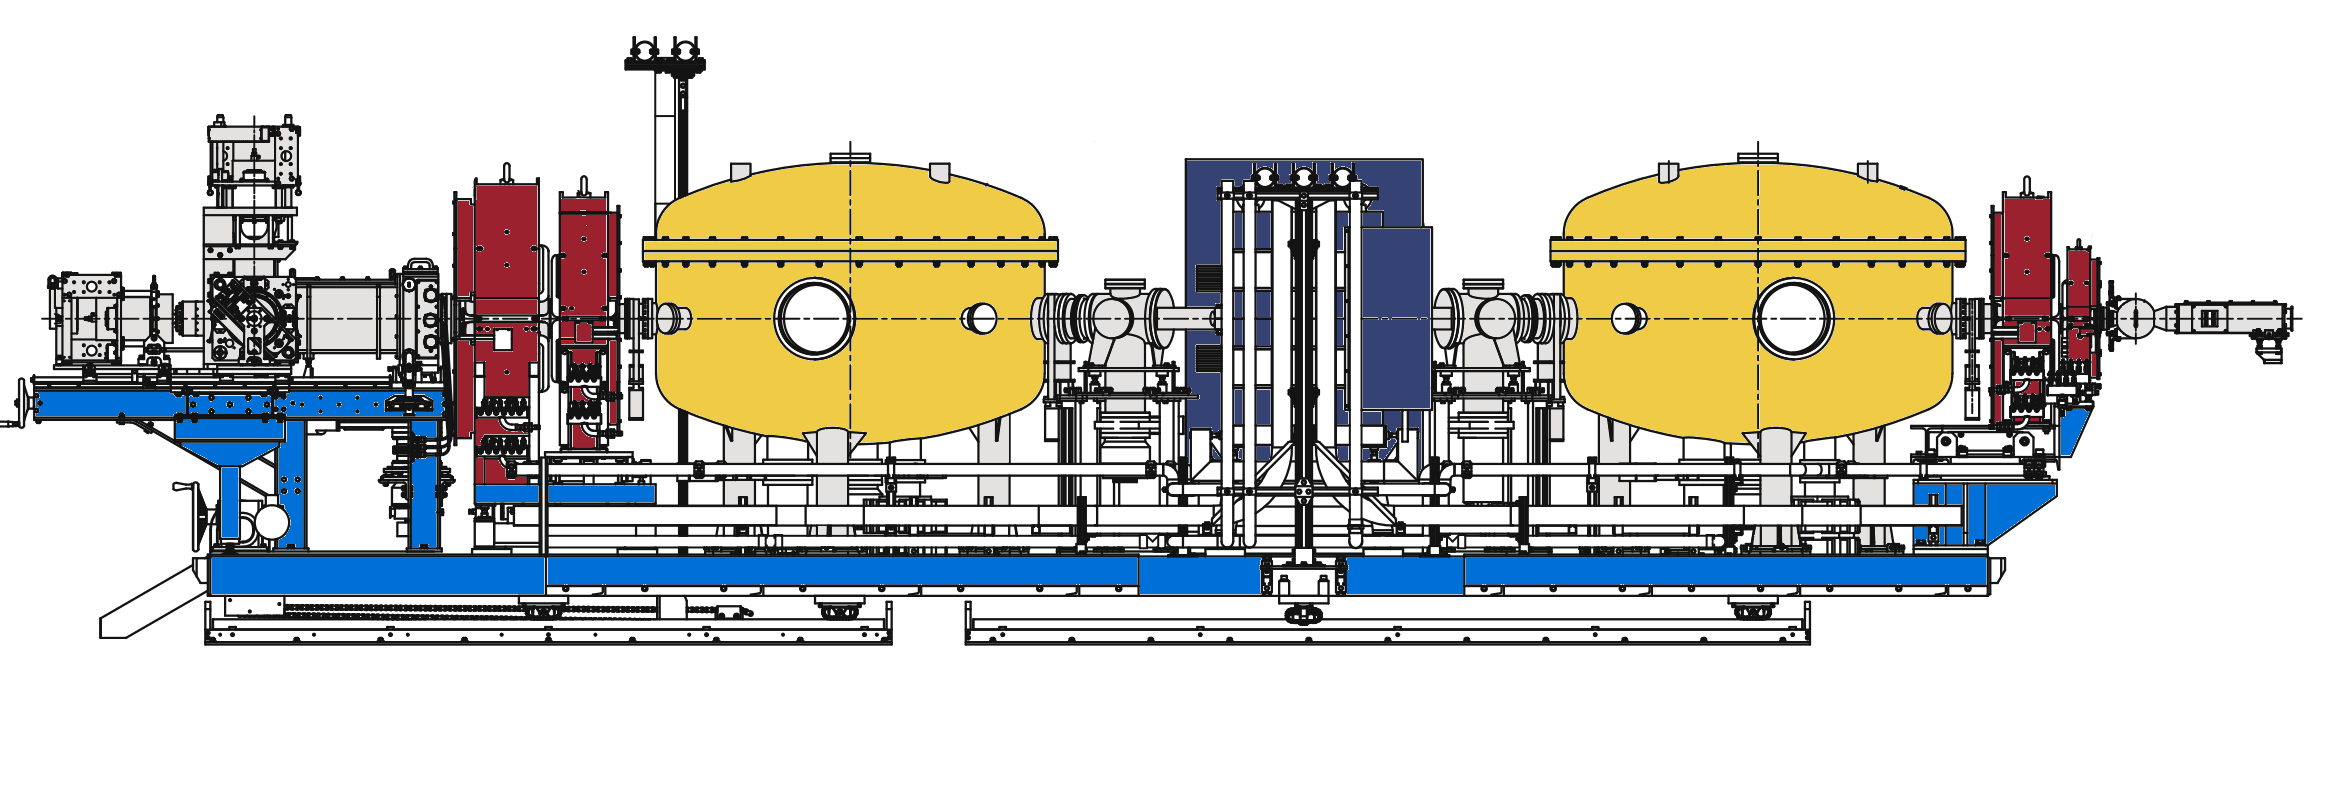
\includegraphics[scale=0.15]{EMMAprofile.png}  
\caption{A profile view of the EMMA spectrometer.}
\label{EMMAprofile}
\end{figure}

This brief guide explains a comprehensive procedure to install the G4EMMA simulation on Linux systems (or Windows with the Bash shell, which is supported on Windows 10). For other types of systems, the essential procedures are the same, with the main differences between different commands executed in the terminal. 

The G4EMMA simulation is created on the framework of CERN's Geant4 version 9.6.4.p04. Additionally, it uses CERN's ROOT 5.34 program to write results and data. Both these programs are required to use the G4EMMA simulation.

This guide is a work in progress. It is likely that in the future, as the simulation is further improved and expanded, changes will need to be made to the source files and installation procedures.  

In this documentation I use my Windows system (with the Bash shell), but the procedures for Linux are the same. OS X will require slightly different commands, but the procedures are also the same. 

Any section which has an individual's name in the section title such as \filefont{How the program works (Naomi Galinski)} is written entirely by that individual. Their work is consolidated here from previous G4EMMA documentations. 

\begin{figure}[h!]
\centering
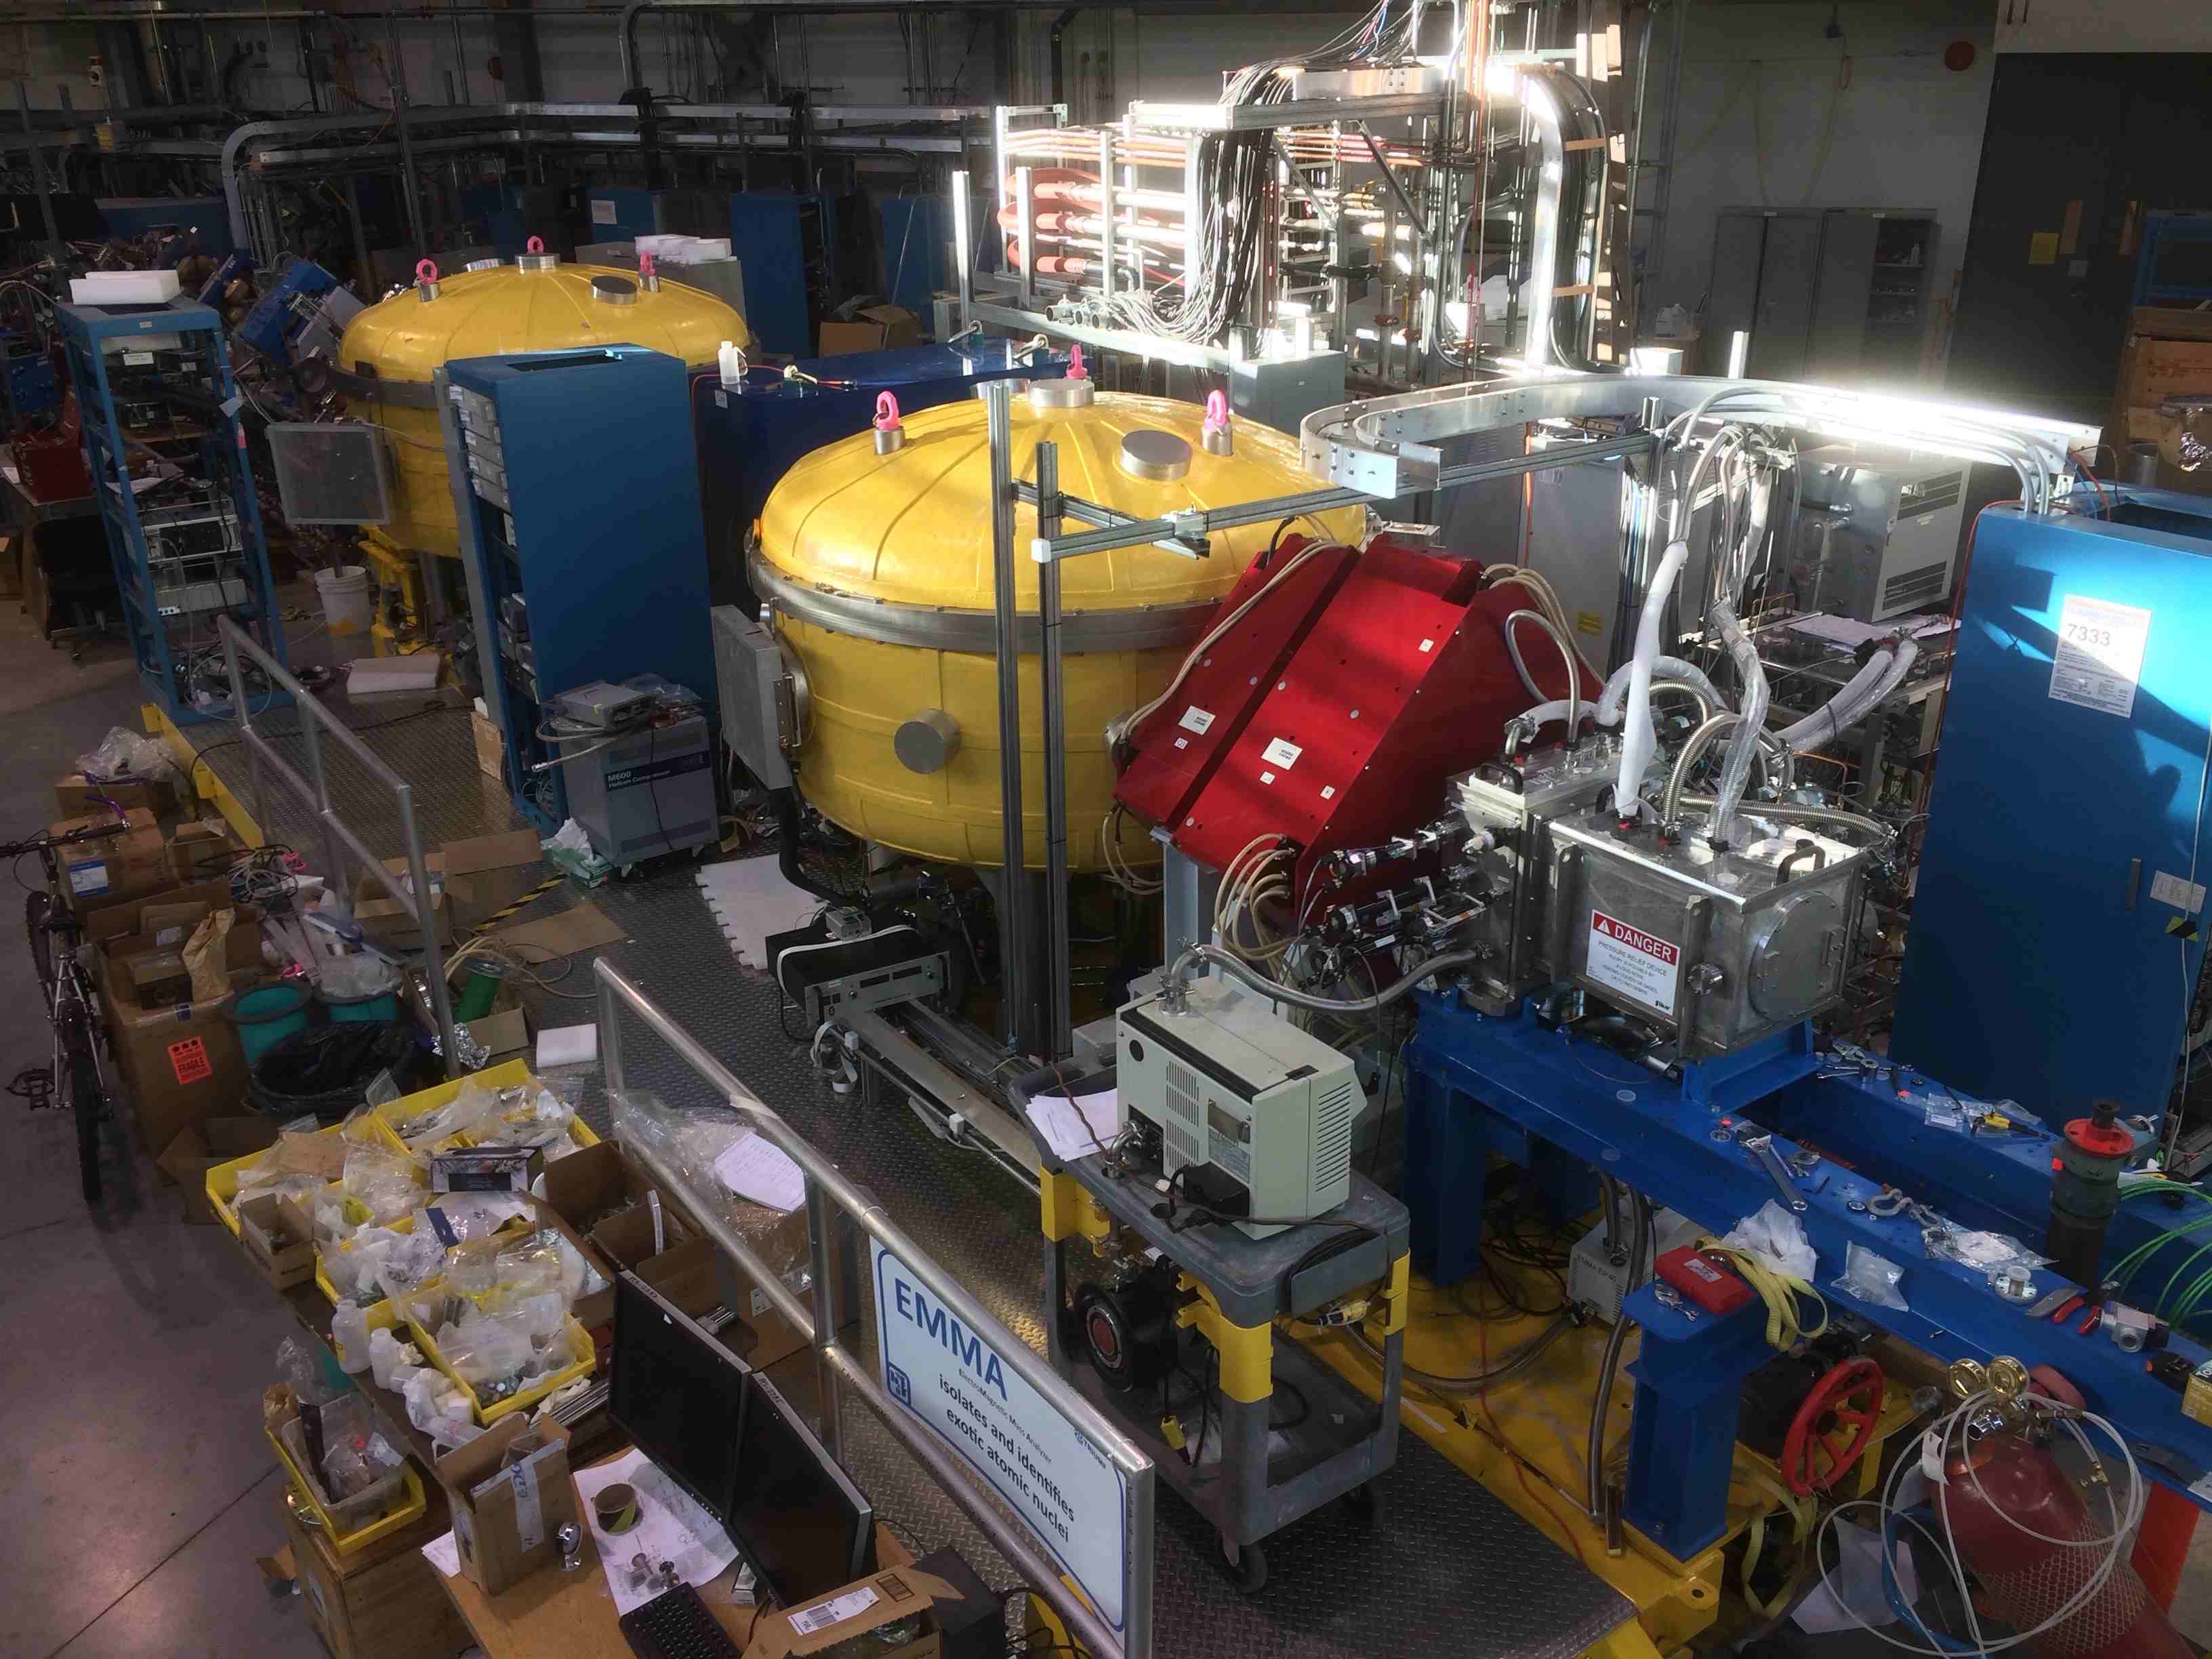
\includegraphics[scale=0.1]{EMMA_1dec2016.jpg}  
\caption{Source: http://davids.triumf.ca/emma.htm.}
\label{EMMA}
\end{figure}

\section{Prerequisites}

Running Geant4, ROOT, and G4EMMA require the usage of various libraries and software. 

I'm not going to include any instructions on how to install Geant 4 and ROOT, since the installs for those programs are fairly well-documented on their respective websites. 

To install EMMA, the command terminal will be used. Open it by searching up \filefont{terminal} in your Windows or Linux search bar. 

\subsection{Required Software}

It is likely that the following (very common) software is already on your system. Use \filefont{apt} to obtain the necessary contents from online. 

Cmake is required to configure. 

\filefont{sudo apt-get install cmake}

Make is required to build.

\filefont{sudo apt-get install make}

The GNU GCC suite is used to compile and build all three programs. Additionally, take extra measures to ensure that the g++ is installed, as the programs of interest operate in C++. You may not necessarily have the problem of g++ not installing properly, but I did - so check anyways. 

\filefont{sudo apt-get install gcc}

\filefont{sudo apt-get install g++}

Finally, you should also have Geant4 and ROOT built and installed. I'm going to assume that you can access the following folders, with the Geant4 and ROOT program files.  

\filefont{[path to]/geant4.9.6.p04} \textit{(source)} \\
\filefont{[path to]/geant4.9.6.p04-build} \textit{(build)} \\
\filefont{[path to]/geant4.9.6.po4-install} \textit{(install)}\\
\filefont{[path to]/root.v5.34} \textit{(source)} \\
\filefont{[path to]/root.v5.34-build} \textit{(build)} 

Depending on how you installed Geant4, you may or may not have another separate \filefont{geant4.9.6.p04-install} folder parallel to the other two, where your files were installed to.  

\subsection{Additional Software for Windows}

If you are using Windows, you will need to download and install an X server (the window manager for Linux) for running the Geant4 EMMA GUI. I recommend Xming - it is available at \hyperref[http://www.straightrunning.com/XmingNotes/]{http://www.straightrunning.com/XmingNotes/}. The latest version is not free, but you can download an older, free version that would work fine. 

Just open the download and follow the given prompts to install. You don't need to install from terminal, because where the Xming directories are doesn't matter and you will not need to change anything - the important thing is that Xming is simply running in the background when you launch the Geant4 EMMA application after you've built it. 

\subsection{Required Libraries}

Geant4 EMMA requires the libraries listed below to successfully run. There is the possibility that some library names may have changed or updated. If, when running the following command, a library is not found, manually search for that library and you will likely find it in an online repository (the library names may have changed slightly from the ones below). Then, you can manually install it using \filefont{apt}. 

To save a lot of time, simply type: \\
\filefont{sudo apt-get install libxerces-c-dev f2c libpthread-stubs0-dev libglew-dev libkrb5-dev libavahi-client-dev libftgl-dev libgsl0-dev libavahi-common-dev libfontenc-dev libxtst-dev libgif-dev libtiff-tools expat freeglut3-dev graphviz libxml2-dev libssl-dev libxmu-dev}

Above are all the library names, each separated by a space. If a problem occurs with any one of them, search them up individually and install the latest version (some of their names may have changed from the above list).

\subsection{Declaring Variables}

Before you begin to build and install the Geant4 EMMA application, you need to declare where your Geant4 and ROOT installations are, so Make knows where to grab the necessary files. 

Open your terminal and enter 

\filefont{nano ~/.bashrc}

This prompts the Nano text editor (in-terminal) to open your \filefont{.bashrc} file, which is the script that is executed every time bash starts up. 

Scroll to the bottom of the file and add a new line to link the location to your \filefont{geant4.sh} file, which is a script that indicates where different parts of your Geant4 install are located. If you have a \filefont{[path to]/geant4.9.6.po4-install} directory, your \filefont{geant4.sh} file is located there within the \filefont{bin} directory. If not, it should be in your source directory, or wherever you ran the install for Geant4. I add

\filefont{source [path to]/geant4.9.6.p04-install/bin/geant4.sh}

Of course, change the above path to wherever your Geant4 is installed, where the \filefont{geant4.sh} file is located. Next, add a line with the same purpose for ROOT: 

\filefont{source [path to]/root.v5.34-build/bin/thisroot.sh}

Again, modify the path to wherever ROOT was installed. Now, add three lines to declare three ROOT variables that are required for ROOT to run, assuming that you haven't moved around anything in the ROOT source directory: 

\filefont{export ROOTSYS=[path to]/root.v5.34} \\
\filefont{export PATH=\$PATH:[path to]/root.v5.34/bin} \\
\filefont{export LD\textunderscore LIBRARY\textunderscore PATH=\$LD\textunderscore LIBRARY\textunderscore PATH:[path to]/root.v5.34/lib}

Finally, for Windows users only, add one more line to inform the X server of which display to run: 

\filefont{export DISPLAY=:0}

Linux users need not worry about this last line. 

After the necessary script has been added, make sure to close (\filefont{Ctrl+X}) and then save (\filefont{Y} when prompted) your .bashrc file. 

\section{Installing G4EMMA}

In my examples I am using the file locations from my Windows system.
 

\subsection{Downloading}

The G4EMMA source code can be downloaded from the GitHub repository as of now; in the future it will probably be available on a permanent server. 

Pay a visit to \hyperref[https://github.com/EMMA-Collaboration/G4EMMA]{https://github.com/EMMA-Collaboration/G4EMMA} and download the repository. When beginning to install, be sure to use the latest branch, which may or may not be \filefont{master}. Older branches sometimes are buggy. Later on, if an install encounters undocumented problems, make sure to double check that your download is complete (or at least if the same download is working on someone else's system).

For demonstration, let's assume that I downloaded the compressed file to \filefont{[path to]}. This can be your \filefont{/opt/} folder, your \filefont{/mnt/c/} disk, or a sub-directory somewhere else where \textbf{the path to the directory does not have any empty spaces}. For Windows users, you may want to consider installing in \filefont{/mnt/c/} because you can directly access the source files via your computer's libraries UI as opposed to in \filefont{opt} or \filefont{home}, since it is thus easier to find and reorganize files that way. 

I downloaded my file as \filefont{/mnt/c/EMMASimulation/G4EMMA.tar.gz}. To unpack the file, I enter the Bash terminal (or just normal terminal for Linux) and enter 

\filefont{cd /mnt/c/EMMASimulation} 

Then, 

\filefont{tar -xzf G4EMMA.tar.gz} 

A directory called \filefont{G4EMMA} should have been created, with all the extracted files. If your file download was in a \filefont{.zip} format, simply unpack it using your computer's default application. 

If you cloned the repository from GitHub instead of downloading it, you don't have to worry about extracting the files; however, keep in mind that any changes or deletions you make during the subsequent compile, build, and install process will also be logged by Git. 

\subsection{Compiling}

First, create a build folder. 

\filefont{cd /mnt/c/EMMASimulation}\\
\filefont{mkdir G4EMMA-build} 

Check the contents of the current directory by typing \filefont{ls}. You should see both the source (\filefont{G4EMMA}) and your newly-created build (\filefont{G4EMMA-build}) folders. Now, switch to your build folder:

\filefont{cd /mnt/c/EMMASimulation/G4EMMA-build} 

and execute the following CMake command, replacing \filefont{[path to]} with the path to your Geant4 source folder:

\filefont{cmake -DGeant4\textunderscore DIR=[path to]/Geant4.9.6.p04}

If successful, you should see the following completion message after a few lines of other checks:  

\filefont{Configuring done\\
-- Generating done\\
-- Build files have been written to: /mnt/c/EMMASimulation/G4EMMA-build}

This step is relatively simple. If all of the previous steps have been done correctly, there should be no errors. If you do encounter any error messages, double check that you have typed the CMake command correctly, and that you are linking to the correct Geant4 source folder. 

\subsection{Building}

When building, it is helpful to know how many computational cores your machine has. You can still build it without knowing, but it is faster if your system has the capacity. 

Run the following \filefont{make} command immediately after compiling, in the build folder: 

\filefont{make -jN}

The \filefont{-jN} part is optional - if you know how many cores your system has, replace N with that number. For example, I would enter \filefont{make -j4} because I have a quad-core system. 

Depending on the speed of your system, the building can take anywhere from 10 seconds to a few minutes. G4EMMA is not a very large application. 

If the build was successful, you will see the following as the final line: 

\filefont{[100\%] Built target EMMAapp}

While the program is building, you will likely see many warning messages indicating that a variable or parameter is ``unused;'' these are non-lethal warnings that simply point to less-than-perfect ways the source code has been written. Simply disregard these. 

However, if you encounter any lethal errors or instances of the build terminating before the completion message, you have a problem. It is possible that different problems may occur on different systems. 

Quickly scan through the whole installation procedure, and make sure everything is executed correctly. You may also find it helpful to test run Geant4 and ROOT with their built-in examples to make sure those programs are working properly too. 

If all else fails, try recompiling and rebuilding the application from the initial download. 

\subsection{Opening G4EMMA}

After building successfully, you should have generated an executable called \filefont{EMMAapp}. If you didn't move this, it should be in your \filefont{G4EMMA-build} directory. 

To run it, go into the build directory

\filefont{cd /mnt/c/EMMASimulation/G4EMMA-build}

Then, simply run with

\filefont{./EMMAapp}

If you are using Windows, make sure Xming is up and running in the background! 

\subsection{Controlling and Starting the Simulation}

To start the simulation, first switch into the folder where the built application (EMMAapp) is located - by default the build folder: 

\filefont{cd [path to]/G4EMMA-build}

And then open the application: 

\filefont{./EMMAapp}

After opening the simulation, your window should look similar to the one in fig. \ref{EMMAapp}. 

\begin{figure}[h!]
\centering
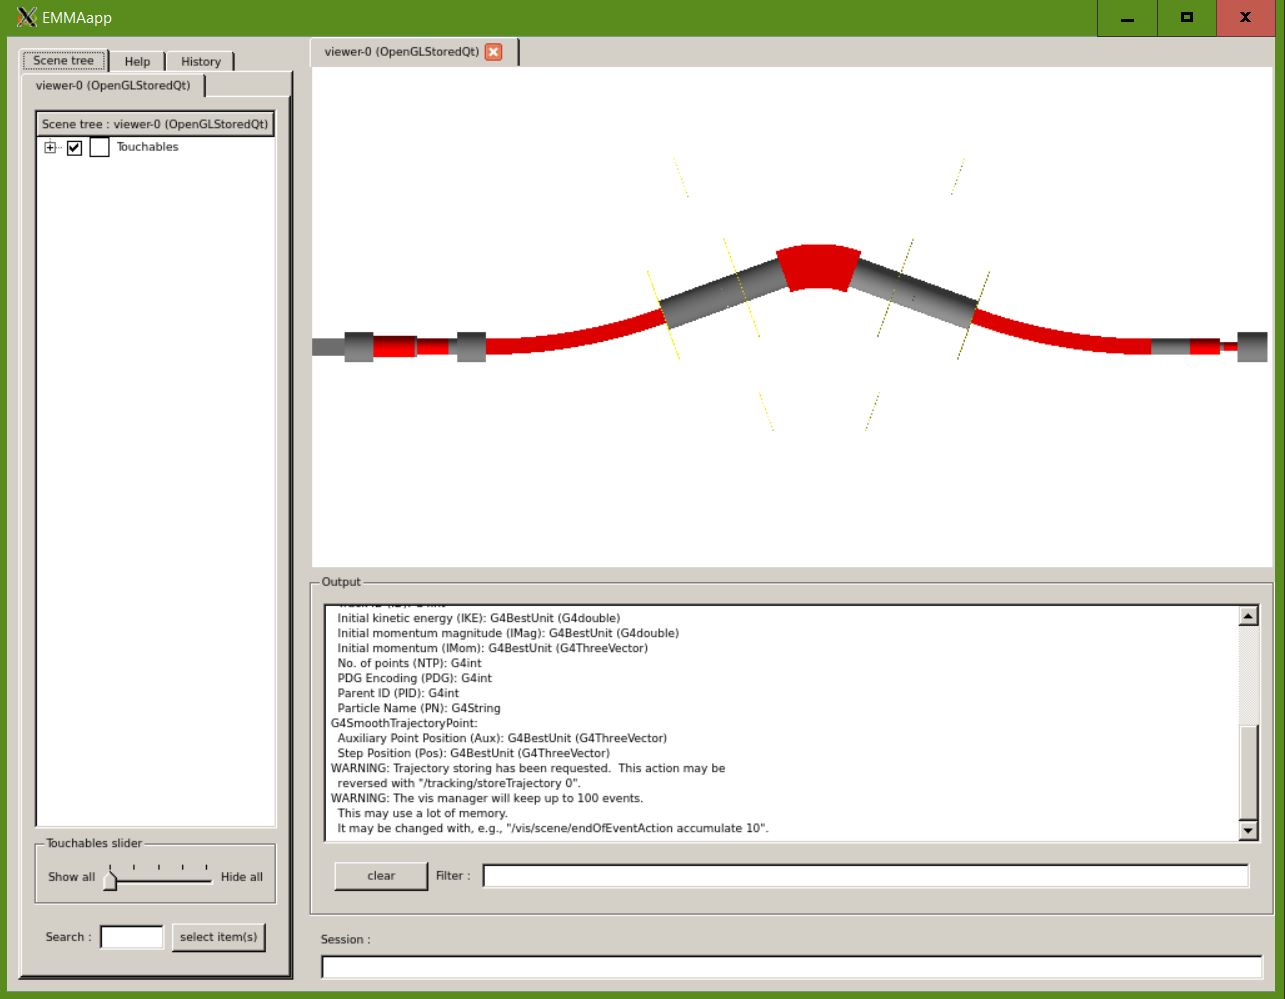
\includegraphics[scale=0.5]{EMMAapp.JPG} 
\caption{The EMMAapp simulation. The command line is at the bottom, labeled ``Session.''}
\label{EMMAapp}
\end{figure}

The simulation parameters are altered from eight .dat files found in \filefont{[path to]/G4EMMA/UserDir/UserInput}. 

The function for each parameter within each file is clearly labeled in their respective files, including units. 

Most importantly, note that centralTrajectory.dat is the information that the spectrometer will use to set its electric and magnetic rigidity, and beam.dat is the information on the beam itself. Therefore, if you want a beam to perfectly pass through the spectrometer, the information in these two files should be the same. 

Before running the simulation for the first time, ensure that the parameters in all the other files are correct, the degraders are right, the slits are open, etc. 

After you edit these files, save them and then start the simulation (you don't need to close these files before starting the simulation). Every time you make changes, however, you must restart the simulation for the changes to take effect. 

\filefont{/mydet/doBeam} is a quick command that simulates the beam scattering through the target, suffering energy loss, and passing through the spectrometer. It does not simulate any reaction.

The simulation is started and controlled through the command line (fig. \ref{EMMAapp}) after EMMAapp is opened. 

\subsubsection{Descriptions of Simulation Commands (Naomi Galinski)}

You will be using the command line to start simulations, visualize the geometry, track particles and make changes to input parameters. I will list some of the most used commands:

\begin{enumerate}
\item \filefont{exit} Exit the program. Note: If you are using ROOT to analyze the data then you must exit the program before you can open the file with ROOT.
\item \filefont{/control/execute visEMMA.mac} Open X11 window, display EMMA and particle tracks.
\item \filefont{/mydet/doBeam} Simulate beam particles through EMMA.
\item \filefont{/mydet/doPrepare} Calculate the energy, position and direction of the beam particles at random reaction depths.
\item \filefont{/mydet/doReaction} Calculate the recoil energy and direction at the reaction depth from the energy and direction of the beam particle calculated with \filefont{/mydet/doPrepare} and transfer reaction kinematics. To simulate recoils you must execute \filefont{/mydet/doPrepare} first.
\item \filefont{/mydet/nEvents n} Change number of events. Substitute \filefont{n} for the number of particles you desire.

\end{enumerate}

If you want to automatically start simulations on startup of the program then uncomment the code around line 220 in \filefont{EMMAapp.cc} and modify as needed.

To view all command line directories type \filefont{ls} in the terminal. You can also type \filefont{ls /directoryname/} to look at a list of sub-directories and commands within. Type \filefont{help commandname}  to get more information about the command.

\section{Output and Results}

\subsection{Output File}

The most important raw output file is in \filefont{[path to]/G4EMMA/UserDir/Results}. 

The file \texttt{fp\_beam.dat} prints, for each particle that makes it to the focal plane, information at the focal plane as well as information on that particle as it left the target. The file \texttt{postTarget\_beam.dat} also contains information on the particle after it leaves the target, but this information is contained in \texttt{fp\_beam.dat} anyways. 

In \texttt{fp\_beam.dat}, there are 11 entries in each line (each line is a particle that hit the focal plane). Each entry is separated from the adjacent one with a comma and space. 

Keep in mind that when speaking about geometries and vectors, we are referring to a Cartesian space with the z-axis pointing downstream along the beam axis, and the x-y plane the same plane as the target and focal plane. The x-direction is the sensitive axis upon which particles will be separated. 

Here are the 11 entries, in this order: 

\begin{enumerate}
	\item Kinetic energy of particle at the focal plane
	\begin{itemize}
		\item declared in the source code as ``Ekin''
	\end{itemize}
	\item Kinetic energy of particle upon leaving the target
	\begin{itemize}
		\item declared in the source code as ``kin''
	\end{itemize}
	\item Polar angle of particle's negative velocity vector at the focal plane
	\begin{itemize}
		\item declared in the source code as ``theta'' and processed and 		displayed as ``theta/deg'' to convert to degree measure
	\end{itemize}
	\item Polar angle of particle's velocity vector upon leaving the target
	\begin{itemize}
		\item declared in the source code as ``ang''
	\end{itemize}
	\item Angle between the z-axis and the particle's velocity vector upon leaving the target projected onto the x-z plane (ie. the velocity vector's azimuth angle measured from the z-axis in the x-z plane)
	\begin{itemize}
		\item declared in the source code as ``angx''
	\end{itemize}
	\item x-component vector of the particle's velocity vector upon leaving the target
	\begin{itemize}
		\item declared in the source code as ``comx''
	\end{itemize}
	\item y-component vector of the particle's velocity vector upon leaving the target
	\begin{itemize}
		\item declared in the source code as ``comy''
	\end{itemize}
	\item x-position of the particle as it hits the focal plane
	\begin{itemize}
		\item declared in the source code as ``worldPos.x()'' and processed and 		displayed as ``worldPos.x()/mm'' to convert to mm measure
	\end{itemize}
	\item x-position of the particle upon leaving the target
	\begin{itemize}
		\item declared in the source code as ``exx''
	\end{itemize}
	\item y-position of the particle as it hits the focal plane
	\begin{itemize}
		\item declared in the source code as ``worldPos.y()'' and processed and 		displayed as ``worldPos.y()/mm'' to convert to mm measure
	\end{itemize}
	\item y-position of the particle upon leaving the target
	\begin{itemize}
		\item declared in the source code as ``why''
	\end{itemize}
	
\end{enumerate}

This information is printed for each particle hit in the focal plane. Hence this file is useful for all sorts of data analysis and can easily be imported (delimited) to an Excel or other similar analysis file. Normally, the data you need is already written to the ROOT file, but I've added these variables in case a need to troubleshoot or analyze things in further detail arises. 

This file is overwritten each run, so save it each time if you want to preserve the raw data. In many cases, all the plots you need are already created on ROOT and saved to a separate .root file. 

You may choose to add, remove, or edit the information that is printed. To do this, you must edit the code (and add or redefine variables) in at least EMMADriftChamberHit.cc. If you want to add or edit any variable that is related to information leaving the target, you also have to edit said variable in EMMASteppingAction.cc and ExternalVariables.hh. 

For reference, the file \texttt{fp\_beam.dat} is opened in EMMAPrimaryGeneratorAction.cc, written to in EMMADriftChamberHit.cc, and called to ROOT in EMMAEventAction.cc. 

The file \texttt{postTarget\_beam.dat} is also opened in EMMAPrimaryGeneratorAction.cc, but written to in EMMASteppingAction.cc. 

The header ExternalVariables.hh links the variables in EMMADriftChamberHit.cc and EMMASteppingAction.cc. Hence variables that are printed can easily be changed via these three files. 



\subsection{ROOT}

After each run in \filefont{[path to]/G4EMMA/UserDir/Results}, there is also a file created called GEMMAoutput.root. This is where ROOT has built plots from the data. 

In the command terminal, switch into the folder

\filefont{cd [path to]/G4EMMA/UserDir/Results}

and open ROOT (if you are using Windows, make sure Xming is running): 

\filefont{root}

Then, enter \filefont{TBrowser browser} to open the ROOT file browser. When you open the file GEMMAoutput.root in TBrowser, you can go in and select various plots you want to see, and edit their appearances. 

There are many different ways to view the ROOT plots, and TBrowser isn't the only one. You should use whichever method you are most comfortable with. 

Alternatively, you can use the ROOT macros (the .C files) in \filefont{[path to]/G4EMMA/UserDir/Results/rootanalysis} to instantly display the ROOT plots. 

\section{How the program works (Naomi Galinski)} \label{howitworks}

I suggest you read the following manuals in parallel to trying to understand how Geant4 and the program works:
\begin{itemize}
\item \hrefcolor{http://amdahl.physics.purdue.edu/geant/applDeveloperMerged.pdf}{Geant4 User's Guide}: This is a shorter manual.
\item \hrefcolor{http://geant4.web.cern.ch/geant4/UserDocumentation/UsersGuides/ForApplicationDeveloper/html/index.html}{Geant4 User's Guide for Application Developers}: This is an extensive manual.
\item \hrefcolor{http://www-geant4.kek.jp/LXR/}{Geant4 Cross Reference}: This is the most useful in searching for Geant4 files, classes, methods, variables, etc. It searches through all Geant4 files including example simulations.
\end{itemize}

\subsection{Main Program}

\filefont{EMMAapp.cc} is the main program. Here we define all user initialization and action classes using \filefont{G4RunManager}. User initialization classes are used during the initialization phase, while user action classes are used during the run. The run manager controls the flow of the program and manages the event loops within a run. 

The visualization is enabled using \filefont{G4VisManager} if Geant4 is compile with OpenGL. The UI session or the interactive mode is enabled using \filefont{G4UImanager}. The UI session allows us to start runs, change certain parameters, open and manipulate a visualization session, and execute macros. Currently, the simulations need to be started via the command line. If you want to automatically start simulations on startup please uncomment and modify lines around line 220.

The verbosity class \filefont{EMMASteppingVerbose} is called which determines how much tracking informations for each event is printed to screen. The amount of screen outputs can be changed by using the terminal command \filefont{/track/verbose n}, where n is the level of verbosity.

Three input files are read in here as well:
\begin{enumerate}
\item \filefont{/UserDir/UserInput/beam.dat}
\item \filefont{/UserDir/UserInput/reaction.dat}
\item \filefont{/UserDir/UserInput/centralTrajectory.dat}
\end{enumerate}
Examples of these files are given in section \ref{sec:input}.

Details on Geant4 main() programs can be found in \hrefcolor{http://geant4.web.cern.ch/geant4/UserDocumentation/UsersGuides/ForApplicationDeveloper/html/ch02.html\#sect.HowToDefMain}{2.1.  How to Define the main() Program}

\subsection{User Initialization Classes}

These are set to \filefont{G4RunManager} through \filefont{SetUserInitialization()} in the main program.

\subsubsection{DetectorConstruction}

This is the detector construction class. \filefont{EMMADetectorConstruction} depends on the following classes:
\begin{itemize}
\item \filefont{EMMADetectorConstructionMessenger}
\item \filefont{EMMADriftChamber}
\begin{itemize}
\item \filefont{EMMADriftChamberHit}
\end{itemize}
\item \filefont{SpectrometerConstruction}
\end{itemize}

In the \filefont{EMMADetectorConstruction} class EMMA is constructed. Physical objects are called volumes in Geant4 and their properties include the geometry, material, position, any magnetic/electric fields and whether the volume is a sensitive detector or not. A sensitive detector is defined using \filefont{G4VSensitiveDetector} and is an abstract class which represents a detector. 

Details on how to define properties of volumes can be found in \hrefcolor{http://geant4.web.cern.ch/geant4/UserDocumentation/UsersGuides/ForApplicationDeveloper/html/ch02s02.html}{2.2.  How to Define a Detector Geometry}.

In \filefont{Construct()} of \filefont{EMMADetectorConstruction.cc} the target, degraders, the detector at the focal plane and Multiwire Proportional Chamber (MWPC) are defined. All materials are defined in \filefont{ConstructMaterials()} and the names of all volumes can be printed to terminal with \filefont{DumpGeometricalTree()}. Some of the properties, such as the target thickness or whether degraders and the MWPC are used, are defined in the \filefont{/UserDir/UserInput/targetDegraders.dat} and \filefont{/UserDir/UserInput/mwpc.dat} input files. The magnetic and electric rigidities of the magnetic and electric dipoles are calculated in the \filefont{CalculateScalingFactors()} method and use the \filefont{/UserDir/UserInput/centralTrajectory.dat} file input parameters.

The \filefont{EMMADetectorConstructionMessenger} implements commands to set values to variables needed to calculate these rigidities. When \filefont{EMMAapp} starts up these values are first read in from \filefont{/UserDir/UserInput/centralTrajectory.dat} in \filefont{EMMAapp.cc}, but can later be changed in the terminal. See section \ref{sec:run} for examples of how to change parameters using the command line. The \filefont{EMMADetectorConstructionMessenger} passes the input file and command line values to \filefont{EMMADetectorConstruction}.

The quadrupole magnets, electric dipoles, magnetic dipoles, slits and walls are constructed in \filefont{SpectrometerConstruction.cc}. The positions of the slits are read in from the \filefont{/UserDir/UserInput/slits.dat} file and are created in the \filefont{buildSlits()} method. The rest of the elements are created in the constructor \filefont{SpectrometerConstruction()}. The geometry and positioning of the elements seem complicated at first. This is why I created a macro called \filefont{visdebug.mac} so that I can display or hide any element that I want. This way you can figure out how each element is rotated and positioned. The electric and magnetic fields are implemented here by calling the \filefont{BDField} classes which in turn call the \filefont{mitray} fortran routines which calculate the fields at different positions located in the \filefont{fortran} folder.

If you make any changes to the names of the volumes in \filefont{EMMADetectorConstruction.cc} or \filefont{SpectrometerConstruction.cc} make sure the correct names are used in \filefont{EMMASteppingAction.cc} (described later). You can also check if there are any overlapping volumes by commenting out the \filefont{fCheckOverlaps=false;} line in the constructors located near the top of both classes. On start up of the program overlap information for each element will be printed to screen.

The detector at the focal plane is defined as a sensitive detector. The \filefont{EMMADriftChamber} class tells the simulation what to do when a particle enters the detector. It uses the information from the steps along the particle track. The kinetic energy, momentum, local position (w.r.t. the volume) and world position (w.r.t. the experimental hall) of each step in the detector are extracted in the \filefont{ProcessHits()} method. The \filefont{Print()} method in the \filefont{EMMADriftChamberHit} class then calls these values and outputs the detector hit information on to screen and a file called \filefont{/UserDir/Results/fp\_beam.dat} or \filefont{/UserDir/Results/fp\_reaction.dat}. Details on sensitive detectors can be found at \hrefcolor{http://geant4.web.cern.ch/geant4/UserDocumentation/UsersGuides/ForApplicationDeveloper/html/ch04s04.html\#sect.Hits.SensDet}{4.4.2.  Sensitive detector}.

\subsubsection{EMMAPhysicsList}

This is the physics list. \filefont{EMMAPhysicsList} depends on the following classes:
\begin{itemize}
\item \filefont{EMMAGeneralPhysics}
\item \filefont{EMMAEMPhysics}
\item \filefont{EMMAMuonPhysics}
\item \filefont{EMMAHadronPhysics}
\item \filefont{EMMAIonPhysics}
\begin{itemize}
\item \filefont{EMMAIonPhysicsMessenger}
\item \filefont{EMMANuclearReactionProcess} NOT USED
\begin{itemize}
\item \filefont{EMMANuclearReactionDataSet} NOT USED
\end{itemize}
\item \filefont{EMMANuclearReactionTwoBody} NOT USED
\item \filefont{G4ScreenedNuclearRecoil} NOT USED
\begin{itemize}
\item \filefont{G4LindhardPartition} NOT USED
\end{itemize}
\end{itemize}
\item \filefont{F04StepMax} NOT USED
\end{itemize}

This is where particles and their physics processes, i.e. interactions with matter, are defined. This is read in once when the program is started and nothing can be changed throughout the session. More information on particle types and physics processes can be found in \hrefcolor{http://geant4.web.cern.ch/geant4/UserDocumentation/UsersGuides/ForApplicationDeveloper/html/ch02s04.html}{2.4.  How to Specify Particles} and \hrefcolor{http://geant4.web.cern.ch/geant4/UserDocumentation/UsersGuides/ForApplicationDeveloper/html/ch02s05.html}{2.5.  How to Specify Physics Processes}.

The files that are not used are eventually going to simulate nuclear reactions including fusion evaporation reactions. Currently we fire the beam and recoil separately. The recoil kinematics are calculated using transfer reaction kinematics. The aim is to have Geant4 simulate the beam and reaction in the same process.

\subsection{User Action Classes}

These are set to \filefont{G4RunManager} through \filefont{SetUserAction()} in the main program.

\subsection{EMMAPrimaryGeneratorAction}

This is the primary generator action. \filefont{EMMAPrimaryGeneratorAction} depends on the following classes:
\begin{itemize}
\item \filefont{EMMAPrimaryGeneratorActionMessenger}
\end{itemize}

Here the particles are called/created and fired with a specified energy, direction and from a specified location. In the constructor \filefont{EMMAPrimaryGeneratorAction()} these variables are initialized. More details on primary generator actions can be found in \hrefcolor{http://geant4.web.cern.ch/geant4/UserDocumentation/UsersGuides/ForApplicationDeveloper/html/ch02s07.html}{2.7. Geant4 General Particle Source}. The \filefont{EMMAPrimaryGeneratorActionMessenger} class is called here. If the beam or reaction properties are changed in the command line the messenger will pass the values to the primary generator action. The constructor also reads in the values from the \filefont{/UserDir/UserInput/alphaSource.dat} file. If the first option in this file is set to 'YES' then an alpha particle is fired instead of the beam particle or recoil.

The methods \filefont{initializeBeamSimulation()}, \filefont{initializeBeamPreparation()} and \filefont{initializeReactionSimulation()} are called when the simulation run commands \filefont{/mydet/doBeam}, \filefont{/mydet/doPrepare} and \filefont{/mydet/doReaction} respectively are used. These methods open the output files and start the simulations using the method \filefont{G4RunManager::GetRunManager()-$>$BeamOn(nEvents)}. The following output files are opened but not written to:
\begin{itemize}
\item \filefont{initializeBeamSimulation()}:
\begin{itemize}
\item \filefont{/userDir/Results/fp\_beam.dat}
\item \filefont{/userDir/Results/postTarget\_beam.dat}
\item \filefont{/userDir/Results/postDegrader1\_beam.dat}
\end{itemize}
\item \filefont{initializeReactionSimulation()}:
\begin{itemize}
\item \filefont{/userDir/Results/fp\_reaction.dat}
\item \filefont{/userDir/Results/postTarget\_reaction.dat}
\item \filefont{/userDir/Results/postDegrader1\_reaction.dat}
\end{itemize}
\item \filefont{initializeBeamPreparation()}:
\begin{itemize}
\item \filefont{/UserDir/BeamSampling/beam.dat} 
\end{itemize}
\end{itemize}
Descriptions of these files can be found in section \ref{sec:outputs}. \filefont{initializeReactionSimulation()}, in addition to creating output files, also opens \filefont{/UserDir/BeamSampling/beam.dat} and reads in the energy, position and momentum of the beam particle at the reaction depth.

When the \filefont{BeamOn()} method of \filefont{G4RunManager} is invoked \filefont{GeneratePrimaries()} in the primary generator action is invoked first. Here the particle type is chosen and it is given a position, momentum and energy. These all depend on whether you're simulating beam particles, preparation beam particles for reactions, recoils or alpha particles. 

For the preparation beam particles the variable \filefont{prepareBeam=true} and the following is done:
\begin{itemize}
\item a random reaction depth from a uniform distribution is selected
\item the target thickness is updated to be equal to the reaction depth
\end{itemize}

If you're simulating the beam all the way through EMMA then the variable \filefont{simulateReaction=false}. In this case the target thickness is kept the original thickness. For both beam particles being prepared for a reaction and passing through EMMA the following is done:
\begin{itemize}
\item the lines in the \filefont{if (simulateReaction==false \&\& !useAlphaSource)} condition are executed
\item the beam particle is chosen
\item the kinetic energy is chosen from a Gaussian distribution given by the mean and fractional energy spread (FWHM)
\item the x and y emission location is chosen from a uniform distribution with the maximum distance given by the beam-spot diameter
\item the z location is set to -0.1 m from the target
\item the emission angle is chosen from a uniform distribution with the maximum angle calculated from the normalized transverse emittance (pi mm mrad)
\end{itemize}
The input parameters from \filefont{/UserDir/UserInput/beam.dat} are used here.

If you're simulating recoils the variable \filefont{simulateReaction=true} and the following is done:
\begin{itemize}
\item the lines in the \filefont{if (simulateReaction)} condition are executed
\item the recoil particle is chosen
\item for each recoil event a new kinetic energy, position and momentum direction of the beam at the reaction depth is called (these were read in from the \filefont{/UserDir/BeamSampling/beam.dat} file)
\item a two body transfer reaction kinematics calculator \filefont{simulateTwoBodyReaction()} is called
\item the reaction kinematics method calculates the energy and momentum direction of the recoil
\end{itemize}
The input parameters from \filefont{/UserDir/UserInput/reaction.dat} are used here.

If you're simulating alpha particles the variable \filefont{useAlphaSource=true} and the following is done:
\begin{itemize}
\item a 6Li(3+) particle is selected and the energy scaled by a factor 1.5 to simulate an $^{4}$He particle (I think this is silly and should be changed)
\item the energy from the \filefont{/UserDir/UserInput/alphaSource.dat} file is selected
\item the emission location is at the origin which is at the target center
\item the momentum direction is selected from a uniform angular distribution between 0 and a maximum angle
\end{itemize}

\subsection{EMMASteppingAction}

The stepping action class tracks the particles. This is done by invoking \filefont{G4Track} and \filefont{G4Step}. Explanations of these can be found in \hrefcolor{http://geant4.web.cern.ch/geant4/UserDocumentation/UsersGuides/ForApplicationDeveloper/html/ch05.html\#sect.Track}{5.1.  Tracking}.

In the \filefont{EMMASteppingAction()} constructor a ROOT histogram for dead hits is created. The ROOT file is created in \filefont{EMMAEventAction}. If a particle hits a wall or a slit the name of the volume hit is added to the histogram. This histogram is created and used only if ROOT is compiled.

The \filefont{UserSteppingAction()} method is called for each event. This method gets the position, kinetic energy and direction of each step along the particle track. For each step it finds/checks in which logical volume the particle is in.

For the reaction preparation beam the following is done:
\begin{itemize}
\item the lines in the \filefont{if (prepareBeam)} condition are executed
\item the beam particle is tracked through the target
\item the kinetic energy, position and direction of the last step point before the particle leaves the target is written to the \filefont{/UserDir/BeamSampling/beam.dat} file
\item the event is terminated
\item note: if the target is too thin, i.e. smaller than the step length, the beam particle might not see the target and pass through to the focal plane. The event will not write anything to file and won't be terminated. This results in fewer lines in the \filefont{/UserDir/BeamSampling/beam.dat} file and the program will crash if you run \filefont{/mydet/doReaction} with the same number of events. You can reduce the number of recoil events to equal the number of lines in the file to bypass this problem.
\end{itemize}

For the beam particles and recoils traveling through EMMA the variable \filefont{prepareBeam=false} and the following is done:
\begin{itemize}
\item the particles are tracked through the target
\item the kinetic energy, angle and x and y position of the last step point before the particle leaves the target is written to the \filefont{/userDir/Results/postTarget\_beam.dat} or \filefont{/userDir/Results/postTarget\_reaction.dat} file
\item the particles are tracked through the degrader if it is used
\item the kinetic energy, angle and x and y position of the last step point before the particle leaves the degrader is written to the\filefont{/userDir/Results/postDegrader1\_beam.dat} or \filefont{/userDir/Results/postDegrader1\_reaction.dat} file
\item if the particle hits a slit or wall then the name of the volume is added to the ROOT histogram and the event is terminated
\end{itemize}

\subsection{EMMAEventAction}

The event action class calls the \filefont{G4EventManager} and it gets the information at the beginning and end of each event. The \filefont{EMMAEventActionMessenger} is called in the \filefont{EMMAEventAction()} constructor. This passes the verbosity level, i.e. how much is printed to screen for each event, to the program if it is changed in the command line. The constructor calls the \filefont{EMMADriftChamberHit} class to access the information of particles that entered the sensitive detector, in other words hit the focal plane. If ROOT is compiled then a ROOT file, some histograms and a tree are created. The ROOT file and tree are created in \filefont{EMMAAnalysisManager} and called into the constructor (this is for this simple purpose an unnecessarily complicated step).

The \filefont{BeginOfEventAction()} method is invoked at the start of every run. This just prints the event number.

The \filefont{EndOfEventAction()} method is invoked at the end of each run if not terminated earlier in the \filefont{UserSteppingAction()} method of \filefont{EMMASteppingAction.cc}. The information from the \filefont{EMMADriftChamberHit} class is called. The \filefont{Print()} method within \filefont{EMMADriftChamberHit} is invoked to print the energy and position of the particle at the focal plane to screen and writes the energy, angle and focal plane position to the \filefont{/UserDir/Results/fp\_beam.dat} or \filefont{/UserDir/Results/fp\_reaction.dat} file. The values are also added to the ROOT histograms and tress.


\section{Function-to-File Quick Reference}

\begin{longtable}[c]{|p{6 cm}|p{6 cm}|}
\hline
Trying to... & Look in... \\
\hline
alter the size or length of the whole spectrometer?                                                    & SpectrometerConstruction                                                                                                         \\ \hline
alter the size of the pipes or thickness of walls?                                                     & SpectrometerConstruction                                                                                                         \\ \hline
redefine or add volumes of the spectrometer, such as vacuums?                                          & SpectrometerConstruction                                                                                                         \\ \hline
change the material of certain aspects of the spectrometer?                                            & SpectrometerConstruction                                                                                                         \\ \hline
change the color or other aesthetic features of the simulation GUI model?                              & SpectrometerConstruction                                                                                                         \\ \hline
rotate or re-orient parts of the spectrometer?                                                         & SpectrometerConstruction                                                                                                         \\ \hline
change the construction or location of the removable slits?                                            & SpectrometerConstruction                                                                                                         \\ \hline
change the size, location, or orientation of any of the electromagnetic fields?                        & SpectrometerConstruction, EMMAElementField, EMMAGlobalField                                                                      \\ \hline
tweak the construction or performance of the first (upstream) quad magnet field?                       & EMMAElementField, EMMAGlobalField, EMMAFieldDebugger, BGField1                                                                   \\ \hline
tweak the construction or performance of the second quad magnet field?                                 & EMMAElementField, EMMAGlobalField, EMMAFieldDebugger, BGField2                                                                   \\ \hline
tweak the construction or performance of the first electric dipole field?                              & EMMAElementField, EMMAGlobalField, EMMAFieldDebugger, BGField3                                                                   \\ \hline
tweak the construction or performance of the magnetic dipole field?                                    & EMMAElementField, EMMAGlobalField, EMMAFieldDebugger, BGField4                                                                   \\ \hline
tweak the construction or performance of the second electric dipole field?                             & EMMAElementField, EMMAGlobalField, EMMAFieldDebugger, BGField5                                                                   \\ \hline
tweak the construction or performance of the third quad magnet field?                                  & EMMAElementField, EMMAGlobalField, EMMAFieldDebugger, BGField6                                                                   \\ \hline
tweak the construction or performance of the fourth (downstream) quad magnet field?                    & EMMAElementField, EMMAGlobalField, EMMAFieldDebugger, BGField7                                                                   \\ \hline
change or add a beam-target collision scattering mechanism?                                            & EMMANuclearReactionDataSet, EMMANuclearReactionTwoBody, EMMANuclearReactionProcess, G4LindhardPartition, G4ScreenedNuclearRecoil \\ \hline
change or tweak how a particle is physically tracked through the simulation?                           & EMMASteppingAction, EMMASteppingVerbose, EMMAAnalysisManager, EMMAEventAction                                                    \\ \hline
alter the way user inputs (beam content, target, physical conditions, etc.) are handled or attributed? & EMMAapp(.cc) {[}in source directory{]}                                                                                           \\ \hline
modify the way or method in which particles are generated and fired?                                   & EMMAEventAction, EMMAPrimaryGeneratorAction, EMMAPrimaryGeneratorMessenger                                                       \\ \hline
edit how detector data is printed and displayed to a ROOT file?                                        & EMMAAnalysisManager                                                                                                              \\ \hline
add or change general detector type, operation, or size?                                               & EMMADetectorConstruction, EMMADetectorConstMessenger, EMMADriftChamber, EMMADriftChamberHit, EMMAIonChamber, EMMAIonChamberHit,  \\ \hline
tweak specifically the operation or characteristics of the PGAC drift chamber?                         & EMMADetectorConstruction, EMMADetectorConstMessenger, EMMADriftChamber, EMMADriftChamberHit, PGACWireParameterization(.hh)       \\ \hline
tweak specifically the operation or characteristics of the ion chamber calorimeter?                    & EMMADetectorConstruction, EMMADetectorConstMessenger, EMMAIonChamber, EMMAIonChamberHit                                          \\ \hline
change or add a method for detectors to collect data?                                                  & EMMADriftChamberHit, EMMAIonChamberHit, EMMADetectorConstruction                                                                 \\ \hline
change or add special materials used by detectors in their construction or operation?                  & EMMADetectorConstruction                                                                                                         \\ \hline
add or change the behavior of EM particles (includes leptons) or related processes?                    & EMMAEMPhysics, EMMAGeneralPhysics, EMMAPhysicsList                                                                               \\ \hline
add or change the behavior of hadrons and their related processes?                                     & EMMAHadronPhysics, EMMAGeneralPhysics, EMMAPhysicsList                                                                           \\ \hline
add or change the behavior of ions (light rare isotopes) and their related processes?                  & EMMAIonPhysics, EMMAGeneralPhysics, EMMAPhysicsList                                                                              \\ \hline
add or change the behavior of muons and taus and their related processes?                              & EMMAMuonPhysics, EMMAGeneralPhysics, EMMAPhysicsList                                                                             \\ 
\hline
\end{longtable}


\section{Appendix}

\subsection{Log of Changes Made Since G4EMMA 1.7}

This section gives an overview of the changes to the source code that have been made by myself in the summer (northern hemisphere) of 2017. This documentation is in comparison to the one by Naomi Galinski's in 2014 titled `` GEMMA1.7documentation(.pdf).'' 

If you have made changes have been made between Naomi's documentation and this present documentation, please add it in either her or my documentation. 

I will describe the changes I made in several key aspects. 

\subsubsection{Documentation and Organization}

I added brief descriptions of source and header files, optimized for Doxygen. In both the \filefont{src} and the \filefont{include} directories, there are two other directories titled \filefont{html} and \filefont{latex}. These were generated by running Doxygen on their respective directories.

Simply use a web browser or \LaTeX\ compiler to view the respective Doxygen files generated. It will include all the documentation for the source and header files I wrote. 

Alternatively, you can simply open up any header or source file itself and look directly at the description, usually located near the beginning of the code. 

Also, keep in mind that my understanding of the code is far from perfect, so if you spot errors or potential improvements, please go ahead and edit the descriptions. 


\subsubsection{Modifications to Structure}

The simulation initially had a problem of particles scattering (fig. \ref{scattering}) out of the target area, straight out of the spectrometer. Granted, some passed through, but the ones that scattered out wasted a lot of time. 

\begin{figure}[h!]
\centering
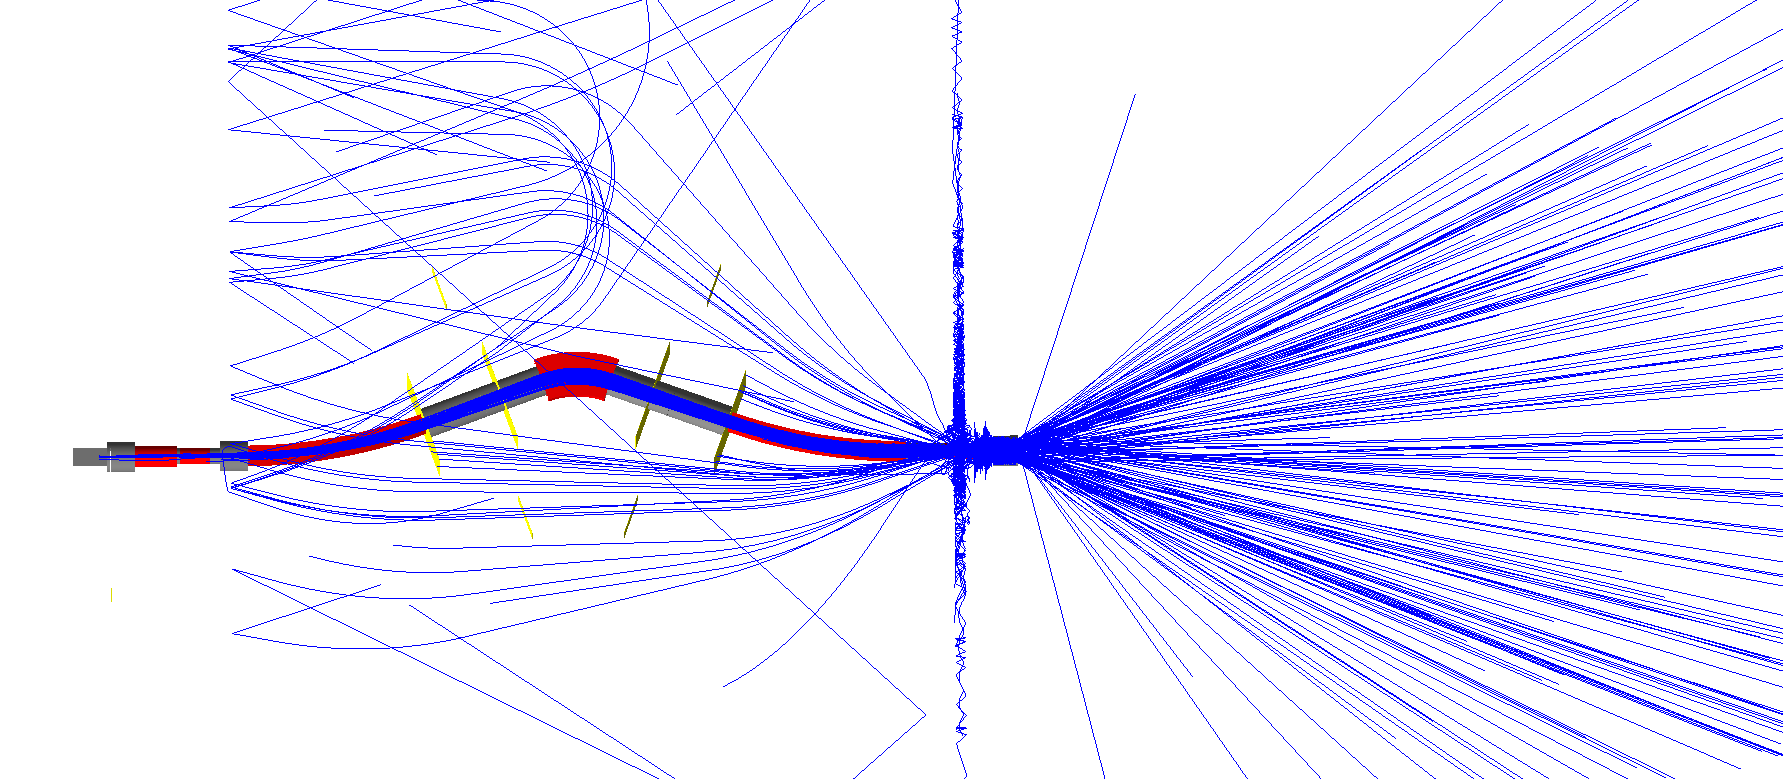
\includegraphics[scale=0.2]{lol.png} 
\caption{This is what the scattering out of the spectrometer initially looked like (particle paths shown in blue).}
\label{scattering}
\end{figure}
 
To fix this problem, the physical structure of the spectrometer had to be modified in the file SpectrometerConstruction.cc. Around Pipe 1, I added metal caps to both the upstream and downstream ends. This contained (fig. \ref{noscattering}) all of the scattering from the target, and ensured that the scattered particles did not take up significant simulation time since their path lengths were now very short inside the pipe before hitting the walls I added. The parts I added are clearly marked in SpectrometerConstruction.cc and named as Pipe1Cap1, Pipe1Cap2, and Pipe1Cap3. They were all just cylinders with varying diameters and lengths. When I added them, they were always on the outside of adjacent pipes or fields, so that they should not have physically affected the path of the particles at all.   

\begin{figure}[h!]
\centering
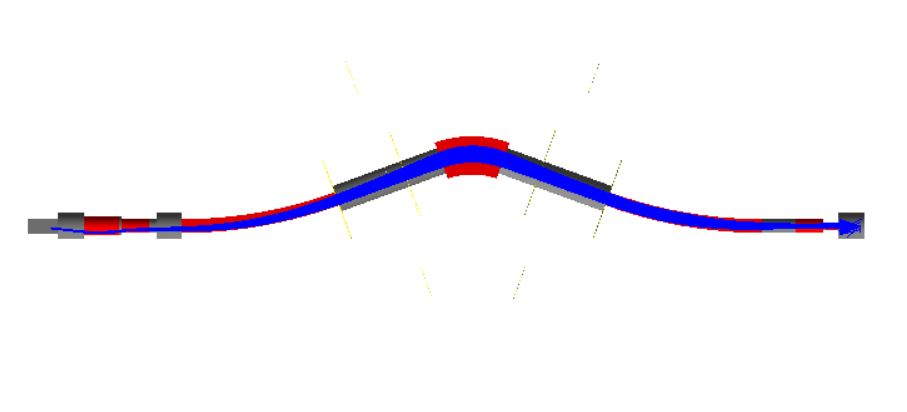
\includegraphics[scale=0.7]{Capture.JPG} 
\caption{After the end caps (walls) were added, costly scattering is considerably reduced.}
\label{noscattering}
\end{figure}

Also, another issue was that some particles would leave the spectrometer through a gap in the pipes before Q3 and reenter the spectrometer after Q4, and hitting the detectors. Obviously such particles shouldn't be part of the experiment results. 

Therefore, I added two more walls to before and after the pair of Q3 \& Q4. Marked as Pipe 11 cap and Pipe 12 cap, they went respectively on the end of Pipe 11 and on the beginning of Pipe 12. Particles now cannot scatter out of the spectrometer and ``skip'' the quadrupole fields on their way to the detectors. Strictly speaking, the cap on the beginning of Pipe 12 isn't necessary since the problematic particles have already been blocked by the first cap at the end of Pipe 11, but at least it aesthetically looks better now. 

\subsubsection{Reproducing Calibration Data}

One of the tests done on the simulation was trying to reproduce the data obtained in the December 2016 run of an argon beam on a gold target, producing Ar 14+ and Ar 13+, and thus creating two central peaks on the focal plane. 

This was generally good on the simulation, but the shape of the peaks were strange and did not model accurately the experimental distribution. An effort was made to localize the source of where the strange distribution on the simulation was coming from. 

A folder called ``Argon FP Analysis'' has been included in the G4EMMA source folder, within it a README file that details what I have done so far, along with all of my data, analysis and graphs. 

I was not successful in localizing the error, and other approaches would have to be used, but this data still yields information on the behavior of particles, and relationships between post-target behavior and focal plane behavior. 



\bibliographystyle{plain}
\bibliography{references}
\end{document}
